% Double-blind IEEE conference paper (IEEEtran). All numbers are taken from the three full-mode notebook runs
% REVISED after audit against the notebooks: search for 'AUDIT' and 'TODO' comments for items that need author action.
% (PICSDB, BIDMC, Fantasia; seed 42). Compile: pdflatex main; pdflatex main  (needs IEEEtran.cls, figures/*)
\documentclass[conference]{IEEEtran}
\usepackage{cite}
\usepackage{amsmath,amssymb,amsfonts}
\usepackage{graphicx}
\usepackage{textcomp}
\usepackage{xcolor}
\usepackage{booktabs}
\usepackage{array}
\usepackage{url}
\usepackage{tikz}
\usetikzlibrary{arrows.meta,positioning,fit,backgrounds}
% figure placeholder: uses figures/<name>.pdf (or .png) if present, otherwise a labelled box
\newcommand{\figph}[3]{\IfFileExists{figures/#1.pdf}{\includegraphics[width=#2]{figures/#1.pdf}}{\IfFileExists{figures/#1.png}{\includegraphics[width=#2]{figures/#1.png}}{\fbox{\parbox[c][#3][c]{0.9\linewidth}{\centering\footnotesize PLACEHOLDER\\\texttt{\detokenize{#1}}}}}}}
\newcommand{\ms}{\,\mathrm{ms}}
\newcommand{\mm}{\,\mathrm{mm}}
\setlength{\textfloatsep}{6pt plus 2pt minus 2pt}
\setlength{\floatsep}{6pt plus 2pt minus 2pt}
\setlength{\intextsep}{6pt plus 2pt minus 2pt}

\begin{document}

\title{Calibrated Probabilistic Forecasting for Latency Compensation of Respiratory Motion: A Closed-Loop Simulation Study on Three Public Cohorts}

\author{\IEEEauthorblockN{Anonymous Authors}
\IEEEauthorblockA{\textit{Affiliation withheld for double-blind review}}}

\maketitle

\begin{abstract}
Latency between sensing and actuation makes a robot that follows a breathing target act on outdated information. We study probabilistic respiratory forecasting as a latency-compensation layer and ask what its predictive uncertainty is good for. Using three public cohorts (9 preterm infants, 50 ICU recordings from 44 patients, 40 healthy young and elderly adults), we train probabilistic LSTM and TCN forecasters and a deep ensemble, calibrate them with split conformal prediction, and drive a simulated one-degree-of-freedom robot that tracks a target derived from the respiratory waveform under observation delays of 0--500~ms, with subject-level held-out evaluation. The ensemble cut forecast error versus persistence by 37--71\% at 300~ms and forecast-based control cut simulated tracking RMSE versus reactive control by 22--45\% at 300~ms and up to 50\% at 500~ms (BIDMC: 4.62$\to$2.65~mm at 300~ms, 5.84$\to$2.92~mm at 500~ms), consistently across cohorts and clearly better than a Kalman baseline. Conformal intervals reached 94--95\% coverage at a nominal 95\%, and coverage did not degrade when models trained on young adults were applied to elderly adults. Predictive uncertainty was an informative risk signal (failure-warning ROC-AUC 0.65--0.73 at 300~ms, well above chance but below respiratory velocity up to 300~ms), edged past velocity only at 500~ms (a small, statistically fragile margin; a forecast-magnitude score did as well or better), and added up to +0.06~AUC to velocity at long delays. Using it as a control gain, in contrast, gave no benefit over trusting the forecast under the validation-tuning grids used, which simplifies the design of such systems. All robot results are simulations driven by a surrogate signal; no physical or clinical validation is claimed.
\end{abstract}

\begin{IEEEkeywords}
respiratory motion forecasting, latency compensation, predictive uncertainty, conformal prediction, tracking failure, uncertainty quantification
\end{IEEEkeywords}

\section{Introduction}
Robot-assisted interventions on moving anatomy, such as needle guidance, radiotherapy tracking and ultrasound positioning, must follow targets displaced by breathing. Sensing, processing, communication and actuation add a latency of tens to hundreds of milliseconds \cite{rCyber}, so a reactive controller aims where the target \emph{was}. A common remedy is to forecast the respiratory state over a horizon equal to the latency and command the robot with the forecast \cite{rArma,rGate,rSoft}.

A point forecast does not reveal when it is reliable. Breathing is quasi-periodic but irregular, and forecasts degrade at pauses, sighs and rhythm changes. A forecaster that outputs a predictive standard deviation $\sigma$ could (i) set how much weight the controller places on the forecast and (ii) warn that tracking is about to fail. Probabilistic respiratory predictors exist \cite{rProb}, but we are not aware of a systematic closed-loop test of whether $\sigma$ helps control or failure anticipation compared with simple non-learned signals such as respiratory velocity.

We study this on three public cohorts with different breathing characteristics: % AUDIT: original said 'fast, irregular'; the notebook EDA (Welch peak of the filtered PICS signal) gives 0.10--0.15 Hz for all nine included infants, i.e. near the 0.1 Hz band edge, which does not support 'fast'. TODO: verify infant respiratory rate (e.g. 0.7--1 Hz expected) and whether the 0.1 Hz high-pass leaves drift in the signal.
preterm infants (the hardest to forecast: 300~ms persistence error 0.80 vs.\ 0.52 and 0.35 in the other cohorts), ICU patients, and healthy young and elderly adults. \emph{Scope:} the databases provide respiration waveforms, not organ displacement, so the target and robot are simulated and millimetre values are simulation units.

\textbf{Contributions.}
\begin{enumerate}
\item \textbf{Forecasting that generalises to held-out subjects.} Probabilistic LSTM/TCN forecasters and a deep ensemble reduce 300~ms error by 37--71\% over persistence on held-out subjects from three cohorts (each cohort trained and tested separately).
\item \textbf{Calibrated uncertainty.} Split conformal intervals achieve 94--95\% coverage at 95\% nominal on held-out subjects and stay close to nominal under a young-to-elderly shift (one small Fantasia split).
\item \textbf{Closed-loop benefit.} In a validated delayed-robot simulation, forecast-based control reduces tracking RMSE by 22--45\% (300~ms) over reactive control and clearly outperforms a Kalman controller at long delays.
\item \textbf{A clear account of what uncertainty is for.} Predictive $\sigma$ is an informative risk signal that edges past velocity only at 500~ms and complements it (a forecast-magnitude score warns better than $\sigma$ in two cohorts), while $\sigma$-gated control variants (blend, rate limit, trigger) are not needed: within the tuning grids used, validation selects trusting the forecast or the weakest gating available.
\end{enumerate}

\section{Related Work}
\emph{Respiratory forecasting.} Adaptive linear filters \cite{rArma}, extended Kalman filters \cite{rJung} and deep sequence models are used to offset system latency. Samadi Miandoab et al.\ \cite{rCyber} compared seven recurrent networks at 115~ms; Wang et al.\ \cite{rWangBiLSTM} showed a Bi-LSTM stays accurate at 400~ms; a review \cite{rZhangReview} finds deep models best above 300~ms but notes inconsistent results over small cohorts and that uncertainty is rarely reported. These give deterministic forecasts evaluated offline on adults; a probabilistic framework \cite{rProb} does not use $\sigma$ in control.
\emph{Uncertainty.} Aleatoric/epistemic decomposition \cite{rKendall}, deep ensembles \cite{rEns}, split conformal prediction \cite{rVovk,rAng,rCuqds} and proper scores \cite{rGneiting,rGuo} provide estimates and intervals. In physiological monitoring, calibrated confidence supports abstention \cite{rBergman}, probabilistic forecasting \cite{rDash} and asynchrony detection \cite{rGMGC}; none feeds forecast uncertainty into an actuator under delay.
\emph{Robot control.} Uncertainty scales limits in probabilistic MPC \cite{rKuo}, plans contact timing \cite{rSURE} and retargets goals under perception lag \cite{rULAG}; adaptive and event-triggered schemes absorb uncertainty into parameters \cite{rWangAdaptive,rKang,rPeddi}, and uncertainty over time predicts failures of learned policies \cite{rFail}. Here, the uncertainty comes from a forecast of an external physiological disturbance, and its value is compared with non-learned alternatives.

\section{Data and Problem Formulation}
\subsection{Datasets}
Table~\ref{tab:data} summarises the cohorts. \textbf{PICS} \cite{rPics,rGee} (PhysioNet \cite{rPhysionet}) holds respiration from preterm infants (abdominal inductance bands, 50~Hz; infant~1 from the bedside monitor, 500~Hz); one infant was excluded by the quality rule (valid fraction $<0.7$), leaving nine. \textbf{BIDMC} contains 8-min ICU recordings (53 records; three excluded by the same rule, leaving 50 records from 44 patients: two patients contribute four records each, and all records of a patient are kept in the same fold). \textbf{Fantasia} contains 20 young and 20 elderly healthy adults; a third-party CSV conversion was verified against the official headers, and one record (f2y02) has a different sampling rate (333~Hz) and is retained. Only the respiration channel is used; annotations are not. All data are public and de-identified.

\begin{table}[t]
\caption{Cohorts and evaluation protocols (all runs: seed 42, full mode; band-pass is 4th-order Butterworth)}
\label{tab:data}
\centering\footnotesize
\setlength{\tabcolsep}{3pt}
% AUDIT: original column widths (0.20/0.23/0.23/0.26) gave an overfull box in the first column; widths rebalanced.
\begin{tabular}{@{}p{0.22\columnwidth}p{0.21\columnwidth}p{0.22\columnwidth}p{0.27\columnwidth}@{}}
\toprule
 & PICS & BIDMC & Fantasia\\
\midrule
Population & preterm infants & ICU patients & healthy adults\\
Subjects used & 9 & 50 rec.\ (44 pts) & 40 (20 y/20 e)\\
Signal length & 60~min & 8~min & 30~min\\
Band-pass & 0.1--3.0~Hz & 0.1--2.0~Hz & 0.1--2.0~Hz\\
Evaluation & 9-fold LOSO (7 train, 1 val, 1 test) & 5-fold, patient-grouped CV & one split: 12 young train, 4 val; test 4 young + 20 elderly\\
Test subjects & 9 & 50 rec. & 24\\
Training & $\le$30 ep., lr $3\!\times\!10^{-3}$ & $\le$40 ep., lr $2\!\times\!10^{-3}$ & $\le$30 ep., lr $3\!\times\!10^{-3}$\\
\bottomrule
\end{tabular}
\end{table}

\subsection{Preprocessing and problem}
Preprocessing is causal: gaps up to 0.25~s are bridged by holding the last sample, longer gaps split the signal, flat-line runs are discarded, a fourth-order Butterworth band-pass (Table~\ref{tab:data}) is applied in one direction with the first 10~s discarded, and the signal is decimated to $f_s=20$~Hz by taking the most recent filtered sample. Samples are normalised with the training-subject mean and standard deviation. With a history of $L=100$ samples (5~s), a forecaster outputs a predictive distribution of $z[t+h]$ for $h\in\{2,4,6,8,10\}$ samples (100--500~ms). At control time $k$ with observation delay $d$ samples the controller sees data only up to origin $o=k-d$, so the forecast horizon equals the delay. Unit tests confirmed no window leakage, training-only normalisation and exclusion of invalid segments.

\section{Methods}
\begin{figure*}[t]
\centering
\resizebox{0.92\textwidth}{!}{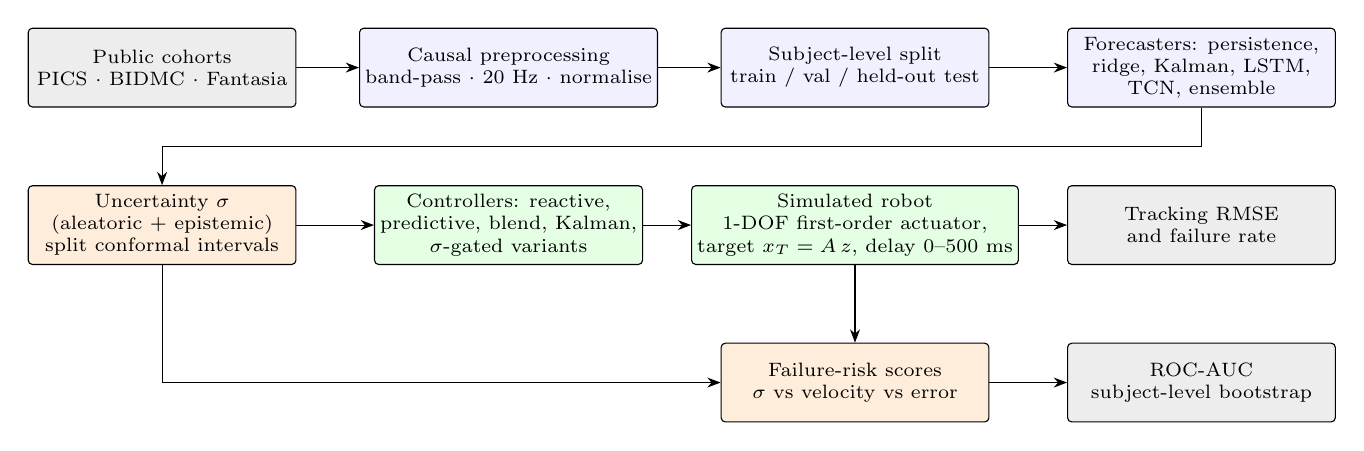
\begin{tikzpicture}[font=\scriptsize,>=Stealth,
 b/.style={draw,rounded corners=1.5pt,align=center,minimum height=10mm,minimum width=34mm,inner sep=2pt,fill=blue!6},
 u/.style={b,fill=orange!14},r/.style={b,fill=green!10},o/.style={b,fill=gray!14}]
\node[o](A) at (0,0){Public cohorts\\PICS $\cdot$ BIDMC $\cdot$ Fantasia};
\node[b](B) at (4.4,0){Causal preprocessing\\band-pass $\cdot$ 20~Hz $\cdot$ normalise};
\node[b](C) at (8.8,0){Subject-level split\\train / val / held-out test};
\node[b](D) at (13.2,0){Forecasters: persistence,\\ridge, Kalman, LSTM,\\TCN, ensemble};
\node[u](E) at (0,-2){Uncertainty $\sigma$\\(aleatoric + epistemic)\\split conformal intervals};
\node[r](G) at (4.4,-2){Controllers: reactive,\\predictive, blend, Kalman,\\$\sigma$-gated variants};
\node[r](H) at (8.8,-2){Simulated robot\\1-DOF first-order actuator,\\target $x_T=A\,z$, delay 0--500~ms};
\node[o](I) at (13.2,-2){Tracking RMSE\\and failure rate};
\node[u](J) at (8.8,-4){Failure-risk scores\\$\sigma$ vs velocity vs error};
\node[o](K) at (13.2,-4){ROC-AUC\\subject-level bootstrap};
\draw[->](A)--(B);\draw[->](B)--(C);\draw[->](C)--(D);
\draw[->](D.south)--++(0,-0.5)-|(E.north);
\draw[->](E)--(G);\draw[->](G)--(H);\draw[->](H)--(I);
\draw[->](E.south)|-(J.west);\draw[->](H)--(J);\draw[->](J)--(K);
\end{tikzpicture}}
\caption{Pipeline: causal preprocessing, subject-level held-out forecasting with calibrated uncertainty (LSTM, TCN, ensemble, conformal), simulated target and delayed first-order robot, five controllers plus $\sigma$-gated variants, tracking metrics and failure-risk evaluation.}
\label{fig:pipeline}
\end{figure*}
\subsection{Forecasters and uncertainty}
\emph{Baselines:} persistence; ridge regression on the 100-sample window (increments, penalty chosen on validation); and a constant-velocity Kalman filter % AUDIT: notebook logs: kalman_q_r=(100,0.001) in all 5 BIDMC folds and in Fantasia; PICS folds 0 and 7 (100,0.001), folds 1--6 (0.01,1) = opposite corner. TODO: widen KF grid and re-run, or keep this caveat.
(noise chosen on validation; the selected values lay at a corner of the search grid in every fold we inspected, so this baseline may be under-tuned). \emph{Learned:} a one-layer LSTM (64 units) and a causal dilated TCN (32 channels, kernel 3), each with a Gaussian head ($\mu_h=z[t]+\Delta_h$, $\sigma_h=\mathrm{softplus}(\cdot)+10^{-3}$) trained with the negative log-likelihood $\tfrac12\log(2\pi\sigma_h^2)+(z[t+h]-\mu_h)^2/(2\sigma_h^2)$; a deterministic TCN; and a deep ensemble of $M=5$ LSTMs whose total variance is the mean member variance (aleatoric) plus the variance of member means (epistemic). Split conformal intervals use a held-out validation block (in Fantasia, separated from the model-selection block by 30~s) with scores $|y-\mu|/\sigma$. We report NLL, 95\% coverage (PICP), interval width and the Spearman correlation between $\sigma$ and absolute error. Coverage guarantees assume exchangeability, which temporal dependence and cross-subject shift violate, so coverage is measured, not assumed.

\subsection{Simulated target, robot and controllers}
\emph{The respiratory waveform is not organ displacement.} The target is $x_T[k]=A\,z[k]$ with an assumed amplitude $A=5$~mm after normalisation (sensitivity at 2 and 10~mm). The robot is a first-order actuator, $v[k]=v[k-1]+\alpha(u[k]-v[k-1])$, with $\alpha=1-e^{-\Delta t/\tau}$, $\tau=0.2$~s, $\Delta t=50$~ms, command saturation at $6A$ and no command delay; the tracking error is $e=x_T-v$ and the first second of each run is excluded. The simulator was validated against the analytic sinusoid response % AUDIT: the PICS notebook's oracle test compares simulate() with itself (tautological, asserts max diff == 0); only the BIDMC/Fantasia notebooks contain the real alignment test. TODO: re-run the v2 oracle test on PICS and then drop the restriction.
(gain within 0.01; Fig.~\ref{fig:sim}) and an oracle forecaster reproduced delay-free tracking (BIDMC and Fantasia runs). All controllers use the same information (measurement and forecast at $o=k-d$):
\begin{itemize}
\item \textbf{Reactive:} $c=z[o]$. \textbf{Predictive:} $c=\mu_h(o)$. \textbf{Fixed blend:} $c=w\mu_h+(1-w)z[o]$, with $w$ from a grid on validation subjects (and $w=0.5$ as reference). \textbf{Kalman:} constant-velocity prediction.
\item \textbf{Uncertainty-aware (UA):} $w_\sigma=\exp(-\sigma_h/(c\,\sigma_{0,h}))$, $\sigma_{0,h}$ the median validation $\sigma$; $c$ is selected on validation from $\{0.25,\ldots,8\}$ % AUDIT/TODO: C_GRID max is 8 for PICS and Fantasia and the tuned c sits at 8 (fold 0 Fantasia, all delays; PICS folds 0--2 shown in the log). Re-run with C_GRID extended to 64 as for BIDMC; the UA-vs-predictive gaps (0.12 mm PICS, 0.33 mm Fantasia) will probably shrink toward the BIDMC value (0.03 mm).
(extended to 64 for BIDMC only; larger $c$ means weaker gating). In Fantasia the selected $c$ was the grid maximum at every delay, and in the PICS folds we inspected as well, so the UA gaps reported for those cohorts are upper bounds on the cost of the weakest gating.
\item \textbf{UA-rate / UCPC:} predictive command passed through a $\sigma$-dependent slew-rate limit. \textbf{UA-trigger:} predictive command, switched to a fixed slew limit when $\sigma$ exceeds a validation quantile. Parameters are chosen on validation; ties go to the least constrained setting. In BIDMC this setting is exactly predictive control; in Fantasia it is a very loose slew limit (1.0 normalised unit per step) that still binds in at most 0.2\% of steps, so it is not exactly predictive control.
\end{itemize}
The ensemble is the primary forecaster for all forecast-based controllers.

\subsection{Failure anticipation and statistics}
A tracking failure at time $k+D$ is $\mathbb{1}\{|e[k+D]|>\epsilon\}$, with the lead equal to the delay $D$ and the threshold fixed a priori at $\epsilon=0.2A=1$~mm (sensitivity at 0.5 and 1.5~mm). Risk scores use only information at decision time: ensemble $\sigma$ (total, aleatoric, epistemic), speed $|z[o]-z[o-1]|f_s$, last forecast error, forecast magnitude $|\mu_h-z[o]|$, and a logistic combination of velocity and $\sigma$ fitted on validation subjects (BIDMC, Fantasia). We report pooled ROC-AUC and subject-level paired differences. Metrics are per subject, aggregated by the subject mean with percentile-bootstrap CIs over subjects; controllers are compared with two-sided paired Wilcoxon signed-rank tests \cite{rWilcoxon} with Holm correction \cite{rHolm} within each pre-specified comparison family (25 primary comparisons per cohort). In BIDMC the unit is the record, so the 50 units are not fully independent (two patients contribute four records each). With $n=9$ the smallest attainable exact two-sided $p$ is $2/2^9=0.0039$, so after Holm correction over 25 comparisons no test can fall below $0.098$ in PICS; PICS $p$-values are therefore reported as effect sizes with CIs only.

\section{Results}
\subsection{Forecasting accuracy and calibration}
Table~\ref{tab:forecast} gives the 300~ms mean absolute error. The LSTM, TCN and ensemble beat persistence and the Kalman baseline in every cohort, whereas ridge regression and the Kalman filter are unreliable: in PICS both are worse than persistence (1.04 and 1.00 vs.\ 0.80), while ridge is among the best models in BIDMC and Fantasia. No single learned model dominates: the TCN is best at 300~ms in PICS and BIDMC, ridge and the ensemble in Fantasia; validation-based selection chose ridge at $\le$200~ms and the ensemble or TCN at longer horizons in Fantasia, and mostly TCN variants in BIDMC. The ensemble reduced MAE relative to persistence by 37\%, 58\% and 71\% at 300~ms (PICS, BIDMC, Fantasia).

\begin{table}[t]
\caption{Subject-mean MAE (normalised units) at 300~ms; 95\% bootstrap CIs are in the supplementary tables.}
\label{tab:forecast}
\centering\footnotesize
\begin{tabular}{@{}lccc@{}}
\toprule
Model & PICS & BIDMC & Fantasia\\
\midrule
Persistence & 0.801 & 0.524 & 0.345\\
Ridge & 1.037 & 0.223 & 0.100\\
Kalman (const.\ vel.) & 0.998 & 0.386 & 0.186\\
LSTM (prob.) & 0.516 & 0.226 & 0.104\\
TCN (det.) & 0.438 & 0.192 & 0.113\\
TCN (prob.) & 0.436 & n/r & 0.108\\
Ensemble ($M{=}5$) & 0.501 & 0.218 & 0.101\\
\bottomrule
\end{tabular}
\par\smallskip% TODO: fill BIDMC TCN (prob.) 300 ms MAE from forecast_metrics.csv (it exists in the run but was not in the displayed summary; it must be >= 0.192).
{\footnotesize n/r: not available in the exported run summary; the best-model summary shows TCN (det.) as the lowest-error model at 300~ms in BIDMC.}
\end{table}

Fig.~\ref{fig:forecast} shows example forecasts with intervals and Table~\ref{tab:calib} gives calibration at 300~ms (reliability in Fig.~\ref{fig:calib}). Raw Gaussian intervals were close to nominal in Fantasia (ensemble 95.4\%) and BIDMC (94.3\%), but under-covering in PICS (ensemble 89.1\%, LSTM 87.1\%), where the TCN was well calibrated (95.3\%). Conformal normalised intervals gave 93.9\%, 94.8\% and 95.2\% coverage; in PICS they remained about one point short. The correlation between $\sigma$ and absolute error was moderate (mean over subject--horizon pairs 0.43 PICS, 0.28 BIDMC, 0.35 Fantasia; range 0.04--0.61), so $\sigma$ is informative about error size but far from a perfect error predictor.

\begin{figure}[t]
\centering
\figph{fig07_calibration_coverage}{\linewidth}{2.5cm}
\caption{Empirical versus nominal coverage (left) and mean absolute error versus predicted $\sigma$ (right) at 300~ms on held-out subjects.}
\label{fig:calib}
\end{figure}

\begin{table}[t]
\caption{Calibration at 300~ms: NLL / 95\% coverage (\%), held-out subjects.}
\label{tab:calib}
\centering\footnotesize
\setlength{\tabcolsep}{3pt}
\begin{tabular}{@{}lccc@{}}
\toprule
Model & PICS & BIDMC & Fantasia\\
\midrule
LSTM & 1.28 / 87.1 & 0.16 / 92.8 & $-$0.80 / 94.4\\
TCN & 0.66 / 95.3 & $-$0.01 / 91.2 & $-$0.74 / 94.2\\
Ensemble & 1.04 / 89.1 & 0.10 / 94.3 & $-$0.82 / 95.4\\
Ens.\ + conformal & -- / 93.9 & -- / 94.8 & -- / 95.2\\
\bottomrule
\end{tabular}
\end{table}

\begin{figure}[t]
\centering
\figph{fig05_forecasts_uncertainty}{0.78\linewidth}{2.5cm}
\caption{Ensemble forecasts with 95\% intervals at 100--500~ms for a held-out Fantasia subject (normalised units).}
\label{fig:forecast}
\end{figure}

\subsection{Closed-loop tracking}
Table~\ref{tab:control} and Fig.~\ref{fig:main} give the simulated RMSE. Predictive control reduced the RMSE of reactive control at 300~ms by 21.5\% (PICS), 42.7\% (BIDMC) and 44.6\% (Fantasia), and by 23\%, 50\% and 47\% at 500~ms. The Kalman controller (a plausible but untested explanation is that its constant-velocity model extrapolates noise) was \emph{worse} than reactive control in PICS at all delays and worse than predictive control everywhere.

\emph{Uncertainty-aware blending did not help.} The validation-tuned fixed blend selected $w=1$ (pure forecast) in all five BIDMC folds, and in Fantasia its RMSE is identical to that of predictive control, so it is a duplicate rather than an independent method; in PICS it chose $w=0.8$--0.9 in some folds (RMSE within 0.015~mm of predictive). UA was likewise tuned to the weakest gating available ($c$ at the grid maximum of 64 in all BIDMC folds, and at the maximum of 8 in Fantasia). Even so, UA was worse than predictive control (Table~\ref{tab:stats}): by 0.12~mm [0.05, 0.19] in PICS, 0.030~mm [0.025, 0.035] in BIDMC and 0.33~mm [0.21, 0.49] in Fantasia at 300~ms, and the differences were stable across delays. In BIDMC and Fantasia these degradations are Holm-significant ($p<10^{-3}$). The $\sigma$-gated rate-limit and trigger variants never beat predictive control: in BIDMC the trigger variant tuned to ``never trigger'' in 5/5 folds and UCPC to ``unconstrained'' in 3--5/5 folds (differences $\le$0.006~mm, $p_{\mathrm{Holm}}\ge0.84$); in Fantasia they were 0.01~mm worse (Holm $p\le0.006$), with the constrained mode active in about 0.2\% of steps at most. UA was better than Kalman at 400--500~ms and in PICS and BIDMC at all delays, but tied with Kalman at 300~ms in Fantasia ($+0.02$~mm [$-$0.11, 0.20]) and was \emph{worse} than Kalman there at 100--200~ms ($+0.17$~mm [0.10, 0.27], $p_{\mathrm{Holm}}=3\times10^{-6}$ at 100~ms; $+0.17$~mm [0.06, 0.33], $p_{\mathrm{Holm}}=0.033$ at 200~ms). Thus, within the tuning grids used, the best $\sigma$-gating on validation subjects was no gating or the weakest gating available: with a well-calibrated forecaster the control loop can simply trust the forecast.

\begin{table}[t]
\caption{Simulated tracking RMSE (mm), subject mean, delays 300/500~ms ($A{=}5$~mm).}
\label{tab:control}
\centering\footnotesize
\setlength{\tabcolsep}{2.5pt}
\begin{tabular}{@{}lcccccc@{}}
\toprule
 & \multicolumn{2}{c}{PICS} & \multicolumn{2}{c}{BIDMC} & \multicolumn{2}{c}{Fantasia}\\
Controller & 300 & 500 & 300 & 500 & 300 & 500\\
\midrule
Reactive & 5.53 & 5.77 & 4.62 & 5.84 & 3.56 & 4.62\\
Predictive & \textbf{4.34} & \textbf{4.43} & \textbf{2.65} & \textbf{2.92} & \textbf{1.97} & \textbf{2.43}\\
Fixed blend ($w{=}0.5$) & 4.74 & 4.87 & 3.56 & 4.19 & 2.72 & 3.39\\
Kalman & 5.98 & 6.44 & 3.38 & 5.12 & 2.29 & 3.44\\
UA blend & 4.46 & 4.56 & 2.68 & 2.95 & 2.31 & 2.79\\
UA rate-limit / UCPC & -- & -- & 2.65 & 2.92 & 1.99 & 2.44\\
\bottomrule
\end{tabular}
\par\smallskip{\footnotesize Validation-tuned fixed blend equals predictive within 0.015~mm (PICS: 4.34/4.44 at 300/500~ms). UA-trigger equals UA-rate in Fantasia and predictive in BIDMC.}
\end{table}

\begin{figure*}[t]
\centering
\figph{fig10_11_error_failure_vs_latency}{0.62\textwidth}{3.2cm}
\caption{Simulated tracking RMSE (left) and failure rate (right) versus observation delay for the controllers, subject mean with 95\% bootstrap CIs (Fantasia; in every cohort predictive control has the lowest RMSE, but the Kalman controller ranks differently, e.g.\ worse than reactive in PICS, see Table~\ref{tab:control}).}
\label{fig:main}
\end{figure*}

\begin{table}[t]
\caption{Failure-warning ROC-AUC (pooled windows) at lead = delay (predictive controller, $\epsilon=1$~mm). Velocity+$\sigma$ was not fitted for PICS.}
\label{tab:auc}
\centering\footnotesize
\setlength{\tabcolsep}{4pt}
\begin{tabular}{@{}llccc@{}}
\toprule
Cohort & Score & 100~ms & 300~ms & 500~ms\\
\midrule
PICS & $\sigma$ (ensemble) & 0.687 & 0.652 & \textbf{0.648}\\
 & Velocity & 0.888 & 0.659 & 0.620\\
 & Forecast mag. & 0.802 & 0.715 & 0.647\\
\midrule
BIDMC & $\sigma$ (ensemble) & 0.763 & 0.689 & 0.679\\
 & Velocity & 0.939 & 0.768 & 0.646\\
 & Forecast mag. & 0.871 & 0.760 & 0.686\\
 & Velocity + $\sigma$ & 0.940 & 0.782 & \textbf{0.694}\\
\midrule
Fantasia & $\sigma$ (ensemble) & 0.742 & 0.728 & 0.736\\
 & Velocity & 0.975 & 0.863 & 0.712\\
 & Forecast mag. & 0.933 & 0.899 & 0.788\\
 & Velocity + $\sigma$ & 0.976 & 0.877 & \textbf{0.776}\\
\bottomrule
\end{tabular}
\end{table}

\begin{table}[t]
\caption{Paired RMSE differences, mean [95\% CI] in mm (negative favours UA).}
\label{tab:stats}
\centering\footnotesize
\setlength{\tabcolsep}{2.5pt}
\resizebox{\columnwidth}{!}{%
\begin{tabular}{@{}llcc@{}}
\toprule
Cohort & Comparison & 300~ms & 500~ms\\
\midrule
PICS ($n{=}9$) & UA$-$predictive & +0.12 [0.05, 0.19] & +0.13 [0.07, 0.21]\\
 & UA$-$Kalman & $-$1.52 [$-$2.11, $-$1.07] & $-$1.88 [$-$2.55, $-$1.24]\\
BIDMC ($n{=}50$) & UA$-$predictive & +0.030 [0.025, 0.035] & +0.034 [0.027, 0.042]\\
 & UA$-$Kalman & $-$0.70 [$-$0.80, $-$0.61] & $-$2.16 [$-$2.42, $-$1.91]\\
Fantasia ($n{=}24$) & UA$-$predictive & +0.33 [0.21, 0.49] & +0.36 [0.22, 0.54]\\
 & UA$-$Kalman & +0.02 [$-$0.11, 0.20] & $-$0.65 [$-$0.84, $-$0.46]\\
\bottomrule
\end{tabular}}
\par\smallskip{\footnotesize Holm-adjusted $p<10^{-3}$ for all BIDMC and Fantasia rows except Fantasia UA$-$Kalman at 300~ms ($p=0.22$). PICS: $p_{\mathrm{Holm}}=0.098$ for every row, the floor for $n=9$.}
\end{table}

\subsection{Failure anticipation}
Predictive uncertainty is an informative warning signal, well above chance at every delay; it falls below velocity up to 300~ms and edges past it only at 500~ms. Failure prevalence at 300~ms was 0.62 in BIDMC and 0.43 in Fantasia, because $\epsilon=1$~mm is a tight threshold. Table~\ref{tab:auc} shows the ROC-AUC and Fig.~\ref{fig:roc} the ROC curves. At 300~ms, $\sigma$ reached 0.65 (PICS), 0.69 (BIDMC) and 0.73 (Fantasia), compared with 0.66, 0.77 and 0.86 for velocity; at 100~ms the gap was 0.18--0.23 in favour of velocity (e.g.\ 0.69 vs.\ 0.89 in PICS). Subject-level paired differences in AUC ($\sigma-$velocity) were $-0.23$, $-0.27$ and $-0.30$ at 100~ms and $-0.03$ [$-$0.06, $-$0.004], $-0.12$ [$-$0.16, $-$0.09] and $-0.18$ [$-$0.21, $-$0.15] at 300~ms. At 500~ms the order reversed: $\sigma$ exceeded velocity by $+0.011$ [$-$0.006, 0.024] in PICS, $+0.034$ [0.003, 0.065] in BIDMC and $+0.028$ [0.004, 0.052] in Fantasia (uncorrected $p=0.13$, 0.08, 0.04), a small and statistically fragile advantage, which persisted at $\epsilon=0.5$ and 1.5~mm in all three cohorts (e.g.\ 0.707 vs.\ 0.694 and 0.776 vs.\ 0.732 in Fantasia). A non-learned score computed from the forecast, the forecast magnitude $|\mu_h-z[o]|$, warned better than $\sigma$ at 300--400~ms in all cohorts and at 500~ms in BIDMC and Fantasia (e.g.\ 0.79 vs.\ 0.74 in Fantasia at 500~ms; Table~\ref{tab:auc}), so what $\sigma$ adds beyond the forecast itself is untested. Combining velocity with $\sigma$ added little at short delays (BIDMC 0.940 vs.\ 0.939 at 100~ms) but +0.01 to +0.06 AUC at longer ones (BIDMC 0.78 vs.\ 0.77 at 300~ms, 0.69 vs.\ 0.65 at 500~ms; Fantasia 0.82 vs.\ 0.78 at 400~ms, 0.78 vs.\ 0.71 at 500~ms; pooled point estimates without confidence intervals, and not fitted for PICS), so $\sigma$ may carry some complementary information when forecasts are long.

\begin{figure}[t]
\centering
\figph{fig12_roc_failure}{0.62\linewidth}{2.5cm}
\caption{ROC curves of the risk scores for failure anticipation (Fantasia, predictive controller, 300~ms delay).}
\label{fig:roc}
\end{figure}

\begin{figure}[t]
\centering
\figph{fig14_distribution_shift}{\linewidth}{2.5cm}
\caption{Young-to-elderly shift (Fantasia): error, mean $\sigma$ and coverage per group.}
\label{fig:shift}
\end{figure}

\subsection{Distribution shift, sensitivity and cost}
\emph{Shift (Fantasia, Fig.~\ref{fig:shift}).} Models trained on 12 young adults and tested on 20 elderly adults were not worse than on the 4 young test subjects (ensemble 300~ms MAE 0.095 vs.\ 0.129; mean $\sigma$ 0.134 vs.\ 0.176; raw 95\% coverage 95.4\% vs.\ 95.1\%; conformal 90\% coverage 90.6\% vs.\ 90.2\%), so $\sigma$ tracked the change in difficulty, but elderly breathing here was easier and no harmful shift occurred. The young group is too small for inference. \emph{Actuator lag.} With $\tau=0.1$ and 0.4~s the ordering of controllers was unchanged (UA remained 0.30--0.33~mm above predictive at 300~ms in Fantasia). \emph{Measurement noise} (exploratory, ridge forecaster, noise SD up to 0.1 of the normalised signal): the Kalman controller overtook predictive control at 100--300~ms in Fantasia (2.37 vs.\ 2.61~mm at 300~ms) but not at 400--500~ms. \emph{Cost.} Batch-1 GPU inference took 0.30--0.35~ms per LSTM and 1.8--2.1~ms per TCN window across cohorts (an $M{=}5$ ensemble therefore costs roughly 1.6~ms if its members run sequentially), well below the 50~ms control step.

\begin{figure}[t]
\centering
\figph{fig_sim_validation_sinusoid}{\linewidth}{2.5cm}
\caption{Simulator validation on a sinusoidal target: robot position and error for reactive control at three delays.}
\label{fig:sim}
\end{figure}

\section{Discussion and Limitations}
\emph{Practical implications.} (i) Forecasting is the part that pays off: gains grow with delay and hold in infants, patients and adults alike. (ii) Conformal calibration needs little data (one validation block per fold) and held up under the benign young-to-elderly shift tested here, but it left PICS about one point short of nominal (93.9\%), so intervals should be validated per population before they are used as safety margins. (iii) The forecast mean already carries most of the information a controller needs; shrinking toward a delayed measurement costs more than it saves, so $\sigma$ is better used for monitoring, alerting or slowing down than as a blending weight. (iv) $\sigma$ and velocity are complementary at long delays, where the forecast itself is the dominant error source. These are interpretations, not tested mechanisms.

\emph{Limitations.} (1) The target is simulated from a respiratory surrogate; amplitude, phase, hysteresis and delay of true anatomical motion differ, and millimetre values are simulation units. (2) The robot is a one-degree-of-freedom first-order system; there is no physical or clinical validation. (3) Cohorts are small (9, 50 and 24 test subjects; Fantasia is a single split with 4 young test subjects), recordings are short slices, and two BIDMC patients contribute four records each. (4) Protocols differ across cohorts (band, learning rate, recording length), so cross-cohort comparisons are descriptive. (5) The failure threshold is a fixed engineering choice that yields high prevalence in two cohorts. (6) Conformal guarantees assume exchangeability, violated by temporal dependence. (7) With $n=9$, Holm-corrected tests in PICS cannot reach significance, so non-significance there is not equivalence. (8) The noise sensitivity covers the ridge forecaster only. (9) Data are retrospective and no inference latency was injected. (10) Other uses of $\sigma$ (e.g.\ gating learned end-to-end) were not explored. (11) The UA gate was tuned on a grid whose upper end was binding in PICS and Fantasia, and the Kalman parameters lay at a grid corner, so the UA and Kalman comparisons are conditional on these grids. (12) The PICS run predates later pipeline changes (no UCPC/trigger, no plant or noise sensitivities, no validation-only model-selection table).

\section{Conclusion}
Probabilistic forecasting is an effective, inexpensive latency-compensation layer for respiratory tracking: across three public cohorts it cut simulated tracking error by 22--45\% at 300~ms (up to 50\% at 500~ms), with calibrated intervals that hold on unseen subjects and under a young-to-elderly shift. Predictive uncertainty is an informative risk signal, a marginally better warning than velocity only at 500~ms and a possible complement to velocity at long delays, whereas blending, rate-limiting or triggering the controller with it gave no further gain. Uncertainty is therefore best treated as a monitoring and safety signal on top of a trusting predictive controller, with its added value over simpler forecast-derived scores still to be shown. These findings hold in simulation on a surrogate signal; future work should use measured organ motion, hardware-in-the-loop tests and risk-sensitive controllers trained end-to-end.

\section*{Reproducibility}
Data are public on PhysioNet. Code, configurations, seeds, split manifests and the scripts that generate every table and figure will be released in an anonymised repository during review.

{\footnotesize
\begin{thebibliography}{00}
\bibitem{rCyber} Samadi Miandoab \emph{et al.}, ``Respiratory motion prediction based on deep artificial neural networks in CyberKnife system: A comparative study,'' 2023.
\bibitem{rArma} ``Adaptive prediction of respiratory motion for motion compensation radiotherapy.''
\bibitem{rGate} ``Prediction-based compensation for gate on/off latency during respiratory-gated radiotherapy,'' arXiv:1810.04326.
\bibitem{rSoft} ``Learning-based prediction of soft-tissue motion for latency compensation in teleoperation,'' \emph{CMES}, 2025.
\bibitem{rProb} ``Potential of a probabilistic framework for target prediction from surrogate respiratory motion during lung radiotherapy,'' \emph{Phys.\ Med.\ Biol.}, 2021.
\bibitem{rWangBiLSTM} Wang \emph{et al.}, ``Feasibility of respiration prediction based on deep Bi-LSTM for real-time tumor tracking,'' 2018.
\bibitem{rJung} Jung \emph{et al.}, ``Respiratory motion prediction with extended Kalman filters based on local circular motion model,'' 2013.
\bibitem{rZhangReview} Zhang \emph{et al.}, ``Modeling of artificial intelligence-based respiratory motion prediction in MRI-guided radiotherapy: a review,'' 2024.
\bibitem{rBergman} Bergman and Varma, ``Uncertainty-aware deep learning for reliable cardiovascular monitoring under physical activity.''
\bibitem{rDash} Dash \emph{et al.}, ``PhysioGen-KAN: A transparent and uncertainty-aware probabilistic framework for physiological time-series forecasting,'' 2026.
\bibitem{rGMGC} Wang \emph{et al.}, ``Uncertainty-aware non-invasive patient--ventilator asynchrony detection using latent Gaussian mixture generative classifier with noisy label correction,'' 2025.
\bibitem{rKuo} Kuo \emph{et al.}, ``Uncertainty-aware contact-safe model-based reinforcement learning,'' 2021.
\bibitem{rSURE} Zhang \emph{et al.}, ``SURE: Safe uncertainty-aware robot-environment interaction using trajectory optimization,'' 2026.
\bibitem{rULAG} Anamika J.\ H.\ and Muraleedharan, ``U-LAG: Uncertainty-aware, lag-adaptive goal retargeting for robotic manipulation,'' 2025.
\bibitem{rWangAdaptive} Wang, ``Adaptive control of robot manipulators with uncertain kinematics and dynamics,'' 2016.
\bibitem{rKang} Kang \emph{et al.}, ``Tracking of uncertain robotic manipulators using event-triggered model predictive control with learning terminal cost,'' 2022.
\bibitem{rPeddi} Peddi and Bezzo, ``A decision tree-based monitoring and recovery framework for autonomous robots with decision uncertainties,'' 2023.
\bibitem{rCuqds} ``CUQDS: Conformal uncertainty quantification under distribution shift for trajectory prediction,'' arXiv:2406.12100.
\bibitem{rFail} ``Failure prediction at runtime for generative robot policies,'' arXiv:2510.09459.
\bibitem{rKendall} A. Kendall and Y. Gal, ``What uncertainties do we need in Bayesian deep learning for computer vision?'' in \emph{Proc. NeurIPS}, 2017.
\bibitem{rEns} B. Lakshminarayanan, A. Pritzel, and C. Blundell, ``Simple and scalable predictive uncertainty estimation using deep ensembles,'' in \emph{Proc. NeurIPS}, 2017.
\bibitem{rGneiting} T. Gneiting and A. E. Raftery, ``Strictly proper scoring rules, prediction, and estimation,'' \emph{J. Amer. Stat. Assoc.}, vol. 102, no. 477, pp. 359--378, 2007.
\bibitem{rGuo} C. Guo, G. Pleiss, Y. Sun, and K. Q. Weinberger, ``On calibration of modern neural networks,'' in \emph{Proc. ICML}, 2017.
\bibitem{rVovk} V. Vovk, A. Gammerman, and G. Shafer, \emph{Algorithmic Learning in a Random World}. Springer, 2005.
\bibitem{rAng} A. N. Angelopoulos and S. Bates, ``A gentle introduction to conformal prediction and distribution-free uncertainty quantification,'' arXiv:2107.07511, 2021.
\bibitem{rPhysionet} A. L. Goldberger \emph{et al.}, ``PhysioBank, PhysioToolkit, and PhysioNet,'' \emph{Circulation}, vol. 101, no. 23, pp. e215--e220, 2000.
\bibitem{rPics} ``Preterm Infant Cardio-Respiratory Signals Database (PICS),'' PhysioNet, doi:10.13026/C2QQ2M.
\bibitem{rGee} A. H. Gee, R. Barbieri, D. Paydarfar, and P. Indic, ``Predicting bradycardia in preterm infants using point process analysis of heart rate,'' \emph{IEEE Trans. Biomed. Eng.}, vol. 64, no. 9, pp. 2300--2308, 2017.
\bibitem{rWilcoxon} F. Wilcoxon, ``Individual comparisons by ranking methods,'' \emph{Biometrics Bulletin}, vol. 1, no. 6, pp. 80--83, 1945.
\bibitem{rHolm} S. Holm, ``A simple sequentially rejective multiple test procedure,'' \emph{Scand. J. Stat.}, vol. 6, no. 2, pp. 65--70, 1979.
\end{thebibliography}}

\end{document}